\documentclass[tikz]{standalone}
\usetikzlibrary{arrows}
\usetikzlibrary{arrows.meta}

\begin{document}

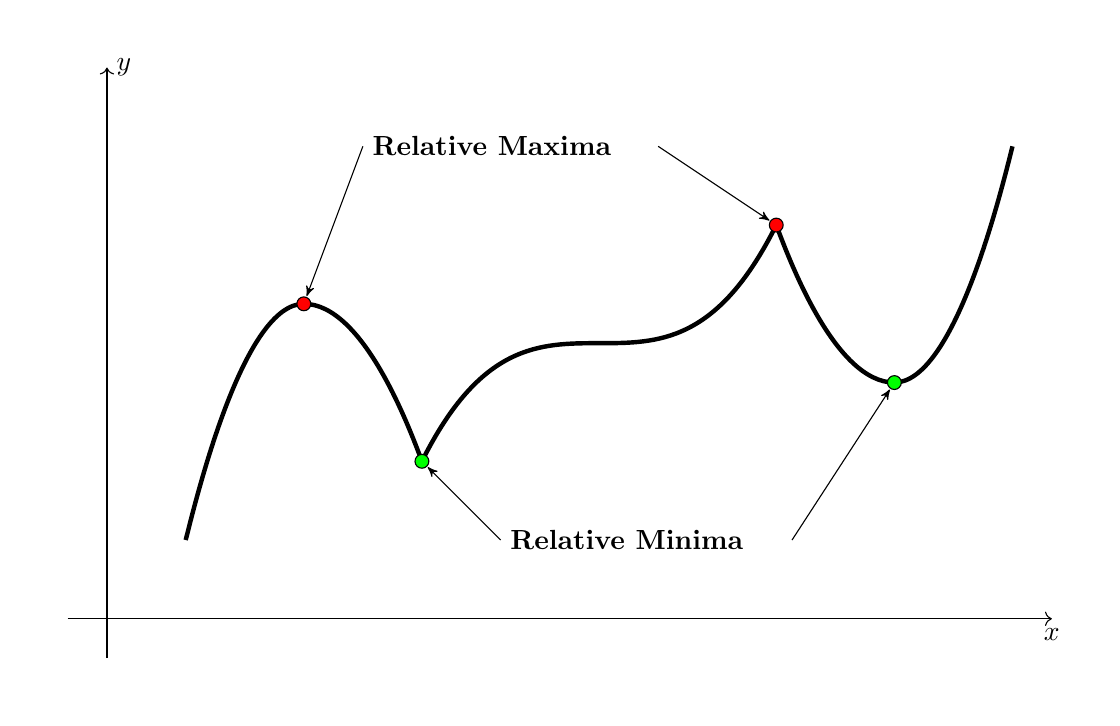
\begin{tikzpicture}[scale = 1]

  \draw[white,fill=white] (-1,-1) rectangle (12.5,7.5);
  \draw[->] (-0.5,0) -- (12,0) node[below] {$x$};
  \draw[->] (0,-0.5) -- (0,7) node[right] {$y$};
      
  % draw curve
  \draw [ultra thick] 
  (1,1) parabola bend (2.5,4) (4,2) 
  .. controls (5.5,5) and (7,2) .. (8.5,5) 
  parabola bend (10,3) (11.5,6);

  % draw points
  \draw [black,fill=red] (2.5,4) circle (2.5pt);
  \draw [black,fill=green] (4,2) circle (2.5pt);
  \draw [black,fill=red] (8.5,5) circle (2.5pt);
  \draw [black,fill=green] (10,3) circle (2.5pt);

  % label extrema
  \draw [<-, >=stealth', shorten <=3pt] (2.5,4) -- (3.25,6) node[right] {\bf Relative Maxima}; 
  \draw [<-, >=stealth', shorten <=3pt] (8.5,5) -- (7,6);
  \draw [<-, >=stealth', shorten <=3pt] (4,2) -- (5,1) node[right] {\bf Relative Minima}; 
  \draw [<-, >=stealth', shorten <=3pt] (10,3) -- (8.7,1);
\end{tikzpicture}
\end{document} 
